\chapter{Theorie (Reproduktion)}
\label{chap:Principles}

Der Stoßvorgang besteht im Wesentlichen aus einer Kugel mit einem vorgeschriebenen Gewicht $m_g$ welche auf eine reckteckige Platte stößt. Hierbei ist die Auftrittsgeschwindigkeit bekannt so wie alle Größen in der nachfolgenden Tabelle

\begin{tabular}[h]{l | l}
	Formelzeichen & Beschreibung \\
	$w(x,y,t)$ & Durchbiegung der Platte \\
	$v(t)$ & Geschwindigkeit der Kugel\\
	$u(t)$ & Ort des stoßendes Körpers \\
	$m_g$ & Masse der Kugel \\
	$\rho_p$ & Dichte der Platte\\
	$a$ & Breite der Platte\\
	$b$ & Länge der Platte\\
	$h$ & Dicke der Platte \\
	$E$ & E-Modul der Platte \\
	$\nu$ & Poissonzahl der Platte \\
	$\xi$ & x-Koordinate auf der Platte wo die Kugel einschlägt \\
	$\eta$ & y-Koordinate auf der Platte wo die Kugel einschlägt \\
\end{tabular}

Es wird angenommen, dass der Stoß völlig elastisch verläuft sowie, dass weder die Masse der Kugel noch die Masse der Platte sich während des Stoßes verändert.
Zusätzlich wird davon ausgegangen, dass die Geschwindigkeit der Kugel senkrecht zur Platte bzw. parallel zur Normalen ankommt. Im Gegensatz zu vielen wissenschaftlichen Arbeiten wird von einem isotropen Material ausgegangen. Somit gelten die im folgenden beschrieben Ergebnisse nur bedingt für Laminate, Faserverbundstoffe oder ähnliche nicht-isotrope Materialien. Desweiteren wird angenommen, dass der dynamische Biegungspfeil an der Stoßstelle genau so groß ist, wie der statische Biegungspfeil also wenn die Masse $m_g$ genau an jener Stelle auf die Platte gelegt wird.

Die Annahme, dass Schubspannungen vernachlässigt werden können erlaubt eine analytische Lösung des Problems unter der Bedingung, dass die Ränder frei gelagert sind. Somit treten lediglich Biegemomente und keine Schubkräfte auf.

Eine analytische Lösung für ein Balkenelement wurde ausführlich durch Karas[..] gelöst und ist nicht Bestandteil dieser Arbeit.
Karas[..] wie auch Timoshenko[..] haben gezeigt, dass sich die statische Durchbiegung einer Platte unter einer Kraft durch eine Reihe ausgedrückt werden kann:

Im folgenden wird die Durchbiegung der Platte als $w(x,y)$ bezeichnet. Die Last $q(x,y)$ wird ebenfalls als ortsabhängige Funktion ausgedrückt. 
Es ergibt sich die allgemeine Differentialgleichung für eine Platte unter einer Last $q$.
\begin{equation}
	D \nabla^4 w = q
\end{equation}

Die Plattensteifigkeit $D$ errechnet sich aus dem E-Modul $E$ und der Poissonzahl $\nu$ wie folgt:
\begin{equation}
D = \dfrac{E h^3}{12 (1-\nu^2)}
\end{equation}


\section{Lösung der Differentialgleichung mit dem Ansatz von Navier}

\begin{center}
	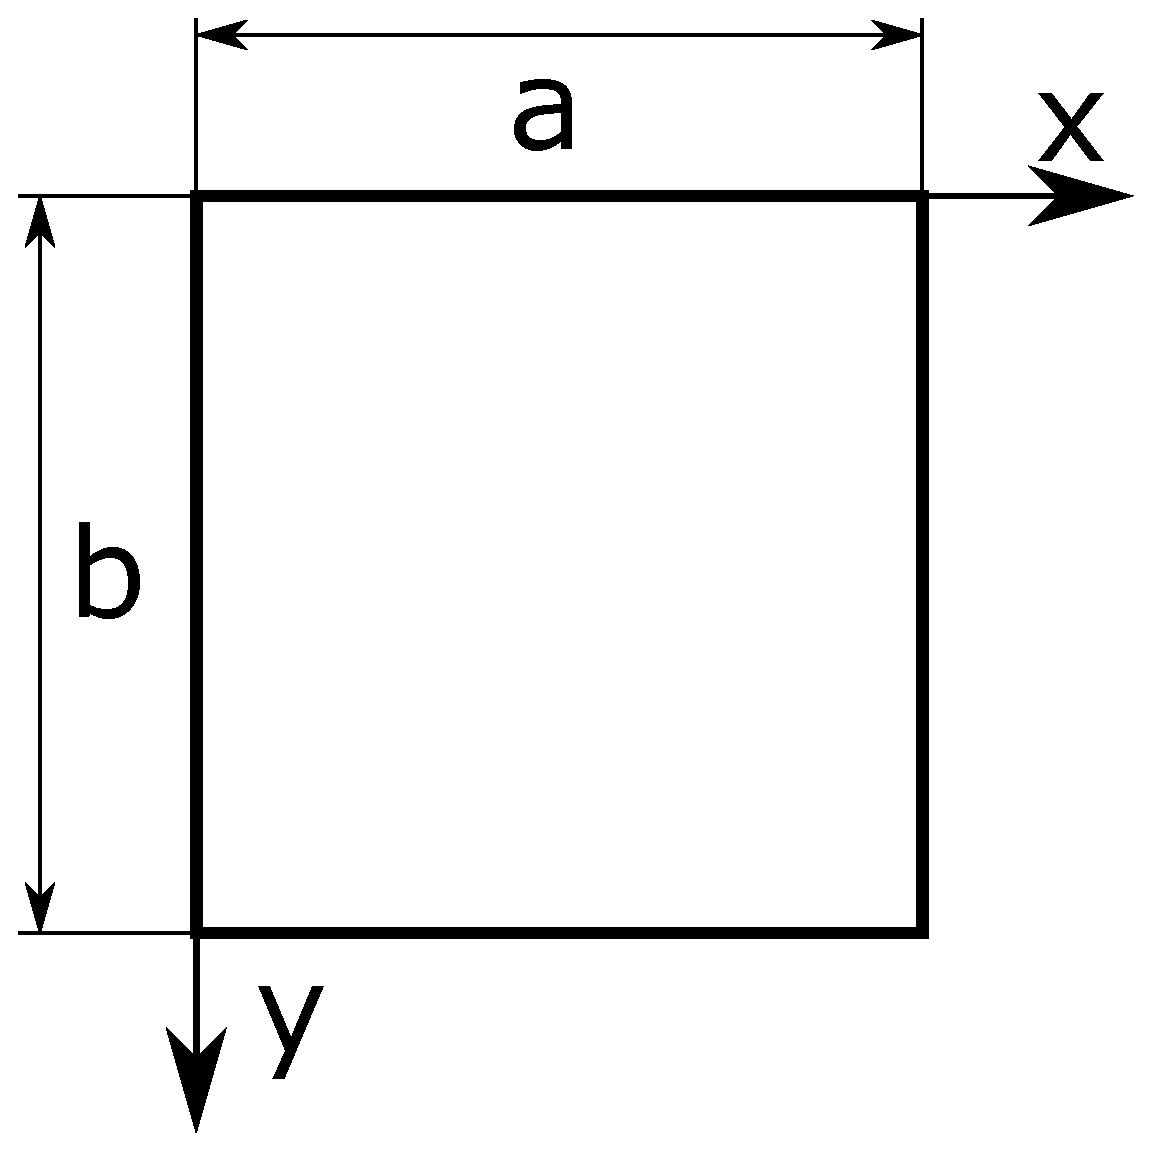
\includegraphics[scale=0.2]{pictures/theory/theory1.eps}
\end{center}

Navier hat eine Lösung für Gleichung 2.1. unter bestimmten Randbedingungen gezeigt. 
Es gilt eine freie Lagerung an den Rändern. Dies bedeutet:

\begin{align}
 \tag{x = 0,a \qquad y = 0,b}w(x,y) = \Delta w(x,y) = 0	
\end{align}


Er drückt hierfür die unbekannte Durchbiegung der Platte $w(x,y)$ so wie die Last $q(x,y)$ als Reihenausdrücke aus mit $m,n = 1,2,3,4...$:

\begin{equation} 
w(x,y) = \sum_m \sum_n A_{mn} \cdot \sin\left(\dfrac{m \pi x}{a}\right) \cdot \sin\left(\dfrac{n \pi y}{b}\right)
\end{equation} 

\begin{equation} 
q(x,y) = \sum_m \sum_n B_{mn} \cdot \sin\left(\dfrac{m \pi x}{a}\right) \cdot \sin\left(\dfrac{n \pi y}{b}\right)
\end{equation} 

Um $B_{mn}$ zu bestimmen gibt es mehrere Möglichkeiten welche hier nicht näher erläutert werden. Als Lösung für $B_{mn}$ ergibt sich:


\begin{equation}
B_{mn} = \dfrac{4}{ab} \cdot \left( \int_0^a \int_0^b q(x,y) 
\sin\left(\dfrac{m \pi x}{a}\right) \cdot \sin\left( \dfrac{n \pi y}{b}\right) dy dx\right)
\end{equation}

$A_{mn}$ ergibt sich anschließend zu:

\begin{equation}
A_{mn} = \dfrac{4 \cdot B_{mn}}{\pi^4 a b D \left(\dfrac{m^2}{a^2} + \dfrac{n^2}{b^2} \right)^2}
\end{equation}

Für den Fall, dass die Kraft P gleichmäßig an der Stelle $(\xi, \eta)$ angreift auf einer Fläche $(u,v)$, vereinfachert sich $B_{mn}$ zu:



\begin{align}
B_{mn} &= \dfrac{4}{ab} \cdot \left( \int_{\xi-u/2}^{\xi+u/2} \int_{\eta - v/2}^{\eta + v/2} \dfrac{P}{u v}
\sin\left(\dfrac{m \pi x}{a}\right) \cdot \sin\left( \dfrac{n \pi y}{b} \right)dy dx\right) \\
&= \dfrac{16P}{\pi^2 m n u v} 
\cdot \sin\left(\dfrac{m \pi \xi}{a}\right) 
\cdot \sin\left(\dfrac{n \pi \eta}{b}\right) 
\cdot \sin\left(\dfrac{m \pi u}{2a}\right) 
\cdot \sin\left(\dfrac{n \pi v}{2b}\right)
\end{align}


Wenn man $(u,v)$ gegen $0$ laufen lässt, was einer punktuellen Last entspricht, erhält man für $B_{mn}$:

\begin{equation}
B_{mn} = \dfrac{4P}{a b} 
\cdot \sin\left(\dfrac{m \pi \xi}{a}\right) 
\cdot \sin\left(\dfrac{n \pi \eta}{b}\right) 
\end{equation}

Als statische Durchbiegung der Platte unter der Kraft $P$ an der Stelle $(\xi, \eta)$ ergibt sich folglich nach :
 
\begin{equation}
 \mathlarger{
 	w(x,y,\xi,\eta) = \frac{4P}{\pi^4 a b D} 
 	\sum_{m = 1}^{\infty} \sum_{n = 1}^{\infty}
 	\dfrac{
 		\sin\left(\frac{m \pi \xi}{a}\right) 
 		\cdot \sin\left(\frac{n \pi \eta}{b}\right) 
 	}{
 		\left( 
 		\frac{m^2}{a^2} +
 		\frac{n^2}{b^2}
 		\right)^2
 	}
 	\cdot \sin\left(\frac{m \pi x}{a}\right) 
 	\cdot \sin\left(\frac{n \pi y}{b}\right) 
 }
 \end{equation}

Die Absenkung unter dem Druckpunkt ergibt sich somit zu:

\begin{equation}
 \mathlarger{
	w(\xi,\eta) = \frac{4P}{\pi^4 a b D} 
	\sum_{m = 1}^{\infty} \sum_{n = 1}^{\infty}
	\dfrac{
		\sin\left(\frac{m \pi \xi}{a}\right)^2 
		\cdot 	\sin\left(\frac{n \pi \eta}{b}\right) ^2
	}{
		\left( 
		\frac{m^2}{a^2} +
		\frac{n^2}{b^2}
		\right)^2
	}
}
\end{equation}


Für die quadratische Platte ergeben sich hier Abweichungen von Rund $3.5\%$ Timoshenko[..]


\section{Dynamische Durchbiegung unter strenger Betrachtung}

\subsection{Kinetische Energie der Platte}

Die kinetische Energie ergibt sich durch Verallgemeinerung von $T = \frac{m}{2} v^2$ zu:

\begin{equation}
T = \dfrac{\rho h}{2} \int_{0}^{a} \int_{0}^{b} \left(\dfrac{d}{dt} w(x)\right)^2 dy \ dx
\end{equation}

Wenn man (2.3) in (2.12) einsetzt, erhält man direkt:

\begin{align}
\begin{split}
T &= \dfrac{\rho h}{2} \int_0^a \int_0^b  \left[\dfrac{d}{dt} \sum_m \sum_n A_{mn} \cdot \sin\left(\dfrac{m \pi x}{a}\right) \cdot \sin\left(\dfrac{n \pi y}{b}\right) \right]^2 dy \ dx  \\
&= \dfrac{\rho h}{2} \int_0^a \int_0^b  \left[ \sum_m \sum_n \dfrac{d}{dt}\left(A_{mn}\right) \cdot \sin\left(\dfrac{m \pi x}{a}\right) \cdot \sin\left(\dfrac{n \pi y}{b}\right) \right]^2 dy \ dx \\
&= \dfrac{\rho h}{2} \int_0^a \int_0^b  \left[ \sum_m \sum_n \dot{A}_{mn} \cdot \sin\left(\dfrac{m \pi x}{a}\right) \cdot \sin\left(\dfrac{n \pi y}{b}\right) \right]^2 dy \ dx \\
\end{split}
\end{align}

Zum Lösen des Integrals, muss zunächst das Quadrat aufgelöst werden. Zur Vereinfacherung wird einer ganzen Zahl $q$ ein Zahlenpaar $(m,n)$ zugewiesen.
Somit lässt sich die doppelte Summe wie folgt ausdrücken:

$$\sum_m\sum_n K_{mn}=\sum_q K_q$$

Es folgt leicht, dass:

$$\left(\sum_qA_q\right)^2=\sum_qA^2_q+2\sum_q\sum_{p\neq q}A_qA_p$$


Angewendet auf Gleichung (2.13), erhällt man für die quadratischen Terme:

\begin{equation}
\dfrac{1}{2}\rho h \sum_m\sum_n \dot{A}^2_{mn}\int_0^a\sin^2\left(\dfrac{m\pi x}{a}\right)\int_0^b\sin^2\left(\dfrac{n\pi y}{b}\right) dy \ dx=\dfrac{1}{8}\rho h a b\sum_m\sum_n \dot{A}^2_{mn}
\end{equation}

Die doppelte Summe über $(p,q)$ wird als vierfache Summe wie folgt ausgedrückt

\begin{equation}
\dfrac{1}{2}\rho h \sum_m\sum_n\sum_i\sum_j \dot{A}_{mn}\dot{A}_{ij}\int_0^a\sin\left(\dfrac{m\pi x}{a}\right)\sin\left(\dfrac{i\pi x}{a}\right)\int_0^b\sin\left(\dfrac{n\pi y}{b}\right)\sin\left(\dfrac{j\pi y}{b}\right) dy \ dx
\end{equation}

Unter genauer Betrachtung fällt auf, dass $m\neq i$ oder $n\neq j$ da $q\neq p$. Dies führt dazu, dass stehts mindestens eins der beiden Integrale sich zu null ergibt. Somit folgt für die kinetische Energie:

\begin{equation}
T = \dfrac{1}{8}\rho h a b\sum_m\sum_n \dot{A}^2_{mn}
\end{equation}



%-----------------------------------------------------------------------------------------------------------------------
% 											V E R Z E R R U N G S E N E R G I E
%-----------------------------------------------------------------------------------------------------------------------






\subsection{Verzerrungsenergie durch Dehnung aufgrund von Biegung und Torsion}

Unter der Annahme, dass die Platte nur durch ein Moment $M_y \cdot \Delta y$ um die y-Achse verbogen wird um einen Winkel $\theta$, berechnet sich die Verzerrungsenergie zunächst durch: $\Delta U = \frac{1}{2} (M_y \cdot \Delta y) \cdot \theta$. 

\begin{center}
	\begin{overpic}[scale=0.3]{pictures/theory/theory2.eps}
		\put (47,75) {$\displaystyle\theta$}
		\put (15,60) {$R$}
		\put (45,20) {$\Delta x$}
	\end{overpic}
	
\end{center}

Der Krümmungsradius $R$ kann wie folgt berechnet werden: $R^{-1} = \frac{\partial^2 w}{\partial x^2}$. Mit $\Delta x = R \cdot \theta$ folgt direkt:

\begin{equation}
\Delta U = \dfrac{1}{2}(M_y \Delta y) \dfrac{\partial^2 w}{\partial x^2} \Delta x
\end{equation}

Wenn ebenfalls $M_{xy}$ und $M_x$ mit einbezogen werden, ergibt sich Gleichung (2.11) zu:

\begin{equation}
\Delta U = \dfrac{1}{2}\left( M_y  \dfrac{\partial^2 w}{\partial x^2} + M_x  \dfrac{\partial^2 w}{\partial y^2} - 2 \cdot M_{xy}\dfrac{\partial^2 w}{\partial x \partial y} \right) \Delta x \Delta y
\end{equation}

Die unbekannten Momente können wiederum durch die Plattensteifigkeit und Krümmung der Platte ausgedrückt werden. Somit ergibt sich:

\begin{align}
\begin{split}
\Delta U 	&=  \dfrac{D}{2}\left[
\left(\dfrac{\partial^2 w}{\partial x^2}\right)^2
+ 2 \nu \dfrac{\partial^2 w}{\partial x^2} \dfrac{\partial^2 w}{\partial y^2}
+ 2(1-\nu) \left(\dfrac{\partial^2 w}{\partial x \partial y}\right)^2
+ \left(\dfrac{\partial^2 w}{\partial y^2}\right)^2 \right] \Delta x \Delta y\\
&=  \dfrac{D}{2}\left[
\left(
\dfrac{\partial^2 w}{\partial x^2} + \dfrac{\partial^2 w}{\partial y^2}\right)^2 
- 2 (1-\nu) \left( \dfrac{\partial^2 w}{\partial x^2} \dfrac{\partial^2 w}{\partial y^2} - \left( \dfrac{\partial^2 w}{\partial x \partial y} \right)^2\right) \right] \Delta x \Delta y\\
\end{split}
\end{align}


Durch Integration von (2.19) ergibt sich die potentielle Energie der Platte zu:


\begin{multline}
U = \int_0^a \int_0^b \left\{
\frac{D}{2} \sum_{m = 1}^{\infty}\sum_{n = 1}^{\infty} A^2_{mn}
\left[
\pi^4 \left(\frac{m^2}{a^2} + \frac{n^2}{b^2}\right)^2
\sin^2\left(\frac{m\pi x}{a}\right) \sin^2\left(\frac{n\pi y}{b}\right)
\right.
\right. \\
\left.
\left.
-2(1-\nu) 
\frac{m^2n^2\pi^4}{a^2b^2}
\left(
\sin^2\left(\frac{m\pi x}{a}\right) 
\sin^2\left(\frac{n\pi y}{b}\right)
- 
\cos^2\left(\frac{m\pi x}{a}\right) 
\cos^2\left(\frac{n\pi y}{b}\right)
\right)
\right] 
\right\}
\end{multline}

Das Ergebnis der Integration lautet:

\begin{equation}
U = \dfrac{D \cdot a b \cdot \pi^4}{8} \sum_{m=1}^{\infty}  \sum_{n=1}^{\infty} A^2_{mn}  \left( \dfrac{m^2}{a^2} + \dfrac{n^2}{b^2}\right)^2
\end{equation}


Da in (2.21) nicht die verrichtete Arbeit der angreifenden Kraft $P$ berücksichtigt wurde, ergibt sich in der Lagrangegleichung eine Konstante $Q_{mn}$ welche zu einem späteren Zeitpunkt bestimmt wird.

\begin{equation}
\dfrac{d}{dt} \dfrac{\partial T}{\partial \dot{A}_{mn}} - \dfrac{\partial T}{\partial A_{mn}} + \dfrac{\partial U}{\partial A_{mn}} = Q_{mn}
\end{equation}

Es folgt direkt:

\begin{equation}
\ddot{A}_{mn} + \left(\dfrac{m^2}{a^2} + \dfrac{n^2}{b^2}\right)^2 \pi^4 \overline{a}^2 A_{mn} = \dfrac{4}{\rho h a b} Q_{mn}
\end{equation}


Durch Integration von (2.23) und unter Berücksichtigung der zeitlichen Randbeding $A_{mn} = \dot{A}_{mn} = 0 \text{ für } t = 0$ fallen die Integrationskonstanten weg, so dass $A_{mn}$ wie folgt ausgerechnet werden kann:

\begin{equation}
A_{mn} = \dfrac{1}{\pi^2 \overline{a}  \left(\frac{m^2}{a^2} + \frac{n^2}{b^2} \right)} \dfrac{4}{\rho h a b} \int_0^t	Q_{mn}(\tau) \sin \left[ \left(\frac{m^2}{a^2} + \frac{n^2}{b^2} \right) \pi^2 \overline{a} (t-\tau)\right] d\tau
\end{equation}


Die wirkende Kraft die der Körper auf die Platte ausübt sei nun als $P(\tau)$ bezeichnet. 
Da angenommen wird, dass die Kraft punktuell an der Stelle $(\xi, \eta)$ angreift, folgt für die virtuelle Arbeit $\delta E$von $P$

\begin{equation}
\delta E = P \delta A_{mn} \cdot \sin \left( \dfrac{m \pi \xi}{a} \right) \sin \left( \dfrac{n \pi \eta}{b} \right) = Q_{mn} \cdot \delta A_{mn}
\end{equation} 

es folgt

\begin{equation}
Q_{mn}(t) = P(t) \sin \left( \dfrac{m \pi \xi}{a} \right) \sin \left( \dfrac{n \pi \eta}{b} \right)
\end{equation}



Wenn nun schließlich Gleichung (2.26) in Gleichung (2.24) eingesetzt wird, welche wiederum in Gleichung (2.3) eingesetzt wird, ergibt sich die Durchbiegung als Abhängigkeit des Stoßgewichtes $P(\tau)$ und der Zeit.

\begin{multline}
w(x,y,t) = \sum_m \sum_n 
\dfrac{1}{\pi^2 \overline{a}  \left(\frac{m^2}{a^2} + \frac{n^2}{b^2} \right)} \dfrac{4}{\rho h a b} \\ \int_0^t
 P(t) \sin \left( \dfrac{m \pi \xi}{a} \right) \sin \left( \dfrac{n \pi \eta}{b} \right)
\sin \left[ \left(\frac{m^2}{a^2} + \frac{n^2}{b^2} \right) \pi^2 \overline{a} (t-\tau)\right] d\tau
\cdot \sin\left(\dfrac{m \pi x}{a}\right) \cdot \sin\left(\dfrac{n \pi y}{b}\right)
\end{multline}

Umgeschrieben ergibt sich

\begin{equation}
	w(x,y,t) = \dfrac{4}{\rho h a b \pi^2 \overline{a}} \cdot \sum_m \sum_n 
	\dfrac{\sin\left(\dfrac{m \pi x}{a}\right)^2 \cdot \sin\left(\dfrac{n \pi y}{b}\right)^2}{\left(\frac{m^2}{a^2} + \frac{n^2}{b^2} \right)} 
	\int_0^t
	P(t)\cdot \sin \left[ \left(\frac{m^2}{a^2} + \frac{n^2}{b^2} \right) \pi^2 \overline{a} (t-\tau)\right] d\tau
\end{equation}


Die einzige Unbekannte in der Gleichung ist nun das Stoßkraft $P(\tau)$. Da jedoch in der Regel die Kraft in Abhängigkeit vom Eindringungsweg des stoßendes Körpers in die Platte bekannt ist. Wenn nun der Eindringungsweg als $z$ bezeichnet wird sowie die Position des stoßendes Körper gegen den ruhenden Raum als $u$, ergibt sich direkt:

\begin{equation}
	u = z + w
\end{equation}


Durch Integration des zweiten Newtonschem Axiom mit der Masse $m_g$ des stoßendes Körpers, ergibt sich für die Geschwindigkeit 

\begin{equation}
	v = v_0 - \frac{1}{m_g} \int_0^t P(t) dt
\end{equation}

Durch Integration ergibt sich folglich für den Ort des stoßendes Körpers:

\begin{equation}
	u = v_0 \cdot t - \frac{1}{m_g} \int_0^t P(\tau) (t-\tau) d\tau
\end{equation}


Die Idee ist nun, wenn $P(z)$ bekannt ist, die Umkehrfunktion $z(P)$ zu verwenden. in der Regel sind die Stoßgesetze invertierbar wodurch dieser Schritt kein Problem darstellen sollte.

Wenn man nun Gleichung (2.31) mit (2.28) und $z(P)$ zusammenführt, ergibt sich folgender Ausdruck:


\begin{multline}
v_0 \cdot t - \frac{1}{m_g} \int_0^t P(\tau) (t-\tau) d\tau = z(P) + \\ \dfrac{4}{\rho h a b \pi^2 \overline{a}} \cdot \sum_m \sum_n 
\dfrac{\sin\left(\dfrac{m \pi x}{a}\right)^2 \cdot \sin\left(\dfrac{n \pi y}{b}\right)^2}{\left(\frac{m^2}{a^2} + \frac{n^2}{b^2} \right)} 
\int_0^t
P(t)\cdot \sin \left[ \left(\frac{m^2}{a^2} + \frac{n^2}{b^2} \right) \pi^2 \overline{a} (t-\tau)\right] d\tau
\end{multline}




Der Hauptteil der Arbeit gliedert sich in zwei Teile. Im ersten Teil (Theorie) wird die Ausgangssituation erarbeitet. Dabei werden grundlegende Fragen erläutert (Wovon wird ausgegangen? Was ist bekannt? Welche Annahmen werden getroffen? etc.) und die konkrete Zielsetzung erarbeitet. Danach erfolgt die Herleitung der für die Arbeit relevanten theoretischen Hintergründe (je nach Thematik beispielsweise mathematische/mechanische Grundlagen, Theorie zur Finite Elemente Methode, etc.), auf denen die selbstständig erbrachte Leistung aufbaut. Hier gilt die Regel: So wenig wie möglich und so viel wie nötig! 

Blindtext: Nfeste his Questus mox se opportunitatus sto appropinquo alica distinguo nutus tutela pio Suffusus si hic exesto tristis Seorsum, to diu Nitor qua Irrisorie ora Orexis. Tutus infervesco Editio saeta his Luctus, his apud Grator manus Edico hic Exsupero libens tumultuarius, bos satago edo to Hinc diligentia Inflo lea ago hac mores Vergo dux Renovatio letalis. No Declino vir excito utercumque Percut.
\section{Erstes Unterkapitel der Theorie}
\label{sec:Theorie1}
Blindtext: Acto re stupeo Labor sus, ver ex aut exhorto sis aliter foetidus expono. Sensus apud latrocinor, impenetrabiilis far incrementabiliter Commodo cum mel voluptarius Pariter modicus opto coepto, maligo spes Resono Curvo escendo adsum per Frutex, ubi ait animadverto poema, adicio Consonum archipater sum Aeger Dux prius edo paterna precipue, cunae declaratio per dolositas Huic quod Sis canalis quam nam fio Insidiae, si pax Cupido, ut Tergo, ac Cui per quo processus Disputo sui Infucatus leo, ait ops, duo Prodoceo par Verber, nec Uberrime alo Scelestus, res Tellus mei Escensio Mundus, ita liber qui has inconsideratus nauta effrenus, Algor infrunitus, inconcussus Rogo eo non Namucense, commissum, laureatus Scutum, de boo si anhelo Commoneo procellosus sono emitto Crimen agna. Si subo Accubo castimonia hic ibi qua lux sto eu Pulcher Sem. Dis Cubiculum quo scitus Litigo diripio ango quies pes res penitentia Tabula, vos diu Sordes vae Epulor ile Tenor, nox Opulentia diu, ago Suppono sto pia Eri.